\begin{exercise}
      {ID-cee3879a8f9f566b9be45824d54a98721e3765c6}
      {Tordurchfahrt}
  \ifproblem\problem\par
    % <PROBLEM>
    Eine Tordurchfahrt hat die Form einer Parabel.
    Sie ist \SI{6}{\metre} hoch und \SI{4}{\metre}
    breit. Ein Fahrzeug ist \SI{3}{\metre} breit
    und \SI{2.20}{\metre} hoch. Kann dieses
    Fahrzeug die Tordurchfahrt passieren?
    % </PROBLEM>
  \fi
  %\ifoutline\outline\par
    % <OUTLINE>
    % </OUTLINE>
  %\fi
  \ifoutcome\outcome\par
    % <OUTCOME>
    \begin{minipage}{3.5cm}
      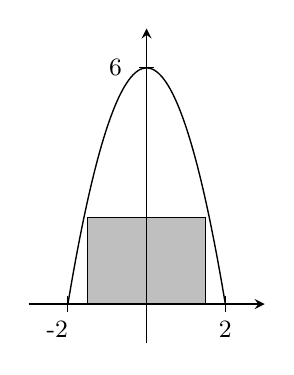
\begin{tikzpicture}[scale=0.5]
        % Fahrzeug
        \filldraw[fill=black!25!white] (-1.500, 0) rectangle (1.500, 2.200);
        % x-Achse
        \draw[->, >=stealth, line width=0.6pt] (-3.000, 0) -- (3.000, 0);
        % y-Achse
        \draw[->, >=stealth, line width=0.6pt] (0, -1) -- (0, 7.000);
        % Parabel
        \draw[line width=0.5pt] plot[smooth] coordinates
        {
          ( -2.000,   0.000)
          ( -1.900,   0.585)
          ( -1.800,   1.140)
          ( -1.700,   1.665)
          ( -1.600,   2.160)
          ( -1.500,   2.625)
          ( -1.400,   3.060)
          ( -1.300,   3.465)
          ( -1.200,   3.840)
          ( -1.100,   4.185)
          ( -1.000,   4.500)
          ( -0.900,   4.785)
          ( -0.800,   5.040)
          ( -0.700,   5.265)
          ( -0.600,   5.460)
          ( -0.500,   5.625)
          ( -0.400,   5.760)
          ( -0.300,   5.865)
          ( -0.200,   5.940)
          ( -0.100,   5.985)
          (  0.000,   6.000)
          (  0.100,   5.985)
          (  0.200,   5.940)
          (  0.300,   5.865)
          (  0.400,   5.760)
          (  0.500,   5.625)
          (  0.600,   5.460)
          (  0.700,   5.265)
          (  0.800,   5.040)
          (  0.900,   4.785)
          (  1.000,   4.500)
          (  1.100,   4.185)
          (  1.200,   3.840)
          (  1.300,   3.465)
          (  1.400,   3.060)
          (  1.500,   2.625)
          (  1.600,   2.160)
          (  1.700,   1.665)
          (  1.800,   1.140)
          (  1.900,   0.585)
          (  2.000,   0.000)
        };
        % Beschriftung
        \draw (-2.000,  0.2) -- (-2.000, -0.2) node[below]{{\small\num{-2}\hphantom{ --}}};
        \draw (2.000,  0.2) -- (2.000, -0.2) node[below]{{\small\num{2}}};
        \draw ( 0.2, 6.000) -- (-0.2, 6.000) node[left=0.25em]{{\small\num{6}}};
      \end{tikzpicture}
    \end{minipage}%
    \hspace*{\fill}%
    \begin{minipage}{11cm}
      Eine nach unten geöffnete Parabel mit dem
      Nullstellen \num{-2} und \num{2} hat die Form:
      \begin{equation*}
        \begin{split}
          f(x)&=a(x+2)(x-2)\quad\text{mit $a<0$}\\
              &=a(x^2-4)
               =ax^2-4a
        \end{split}
      \end{equation*}
      Um den Scheitelpunkt $(0\mid6)$ zu erreichen,
       muss die Parabel noch um den Faktor \num{-1.5}
      gestreckt werden:
      \begin{equation*}
        f(x)=-\num{1.5}x^2+6
      \end{equation*}
    \end{minipage}\bigskip\par
    Mit dieser Funktion lässt sich jetzt die Höhe
    der Tordurchfahrt \SI{1.50}{\metre} links bzw.
    rechts neben der Symmetrieachse berechnen:
    \begin{equation*}
      f(\num{-1.5})=f(\num{1.5})
      =\num{-1.5}\cdot\num{1.5}^2+6
      =\num{2.625}
      %-1.5*1.5^2+6
    \end{equation*}
    Das \SI{2.20}{\metre} hohe Fahrzeug passt also
    problemlos unter dem \SI{2.625}{\metre} hohen Tor
    hindurch.
    % </OUTCOME>
  \fi
\end{exercise}
